\documentclass[11pt]{beamer}
\usetheme{CambridgeUS}
\usecolortheme{seahorse}

\usepackage[utf8]{inputenc}
\usepackage[brazil]{babel}
\usepackage[T1]{fontenc}

\usepackage{amsmath}
\usepackage{amsfonts}
\usepackage{amssymb}
\usepackage{graphicx}
\usepackage{setspace}
\usepackage{ragged2e}


\setbeamertemplate{caption}[numbered]

\author[CETi / IFAM CMC]{Autores \\ Professores: Luiz Claudio, Andreza Barbosa e Joao Victor}
\title{Funções afim e quadrática - (UEA/ENEM)}
%\setbeamercovered{transparent} 
\setbeamertemplate{navigation symbols}{} 
\institute[]{CETi BILÍNGUE GILBERTO MESTRINHO \par INSTITUTO FEDERAL DO AMAZONAS } 
\date{\today} 
\titlegraphic{
\includegraphics[width=0.6\textwidth]{imagens/logo.png}}

%\subject{}

% ---------------------------------------------------------

\begin{document}
\justifying
\onehalfspacing 

\begin{frame}
    \titlepage
\end{frame}

\section{Função afim}

\begin{frame}{ENEM 2023}
    Dirigir após ingerir bebidas alcoólicas é uma atitude extremamente perigosa, uma vez que, a partir da primeira dose, a pessoa já começa a ter perda de sensibilidade de movimentos e de reflexos. Apesar de a eliminação do álcool depender de cada pessoa e de como o organismo consegue metabolizar a substância, ao final da primeira hora após a ingestão, a concentração de álcool (C) no sangue corresponde a aproximadamente $90\%$ da quantidade (q) de álcool ingerida, e a eliminação total dessa concentração pelo fígado ocorre até 12 horas. \textit{Disponível em: http://g1.globo.com Acesso em: 1 dez. 2018 (adaptado).}. \vfill
    \textbf{(continua no próximo slide)}
\end{frame}

\begin{frame}{ENEM 2023 (continuação)}
    Nessas condições, ao final da primeira hora após a ingestão da quantidade q de álcool, a concentração C dessa substância no sangue é expressa algebricamente por:

    \begin{enumerate}[a]
                \item $C = 0,9q$ %
                \item $C = 0,1q$
                \item $C = 1 - 0,1q$
                \item $C = 1 - 0,9q$ 
                \item $C = q - 10$
            \end{enumerate}
\end{frame}

\begin{frame}{ENEM PPL 2017}

    Em um mês, uma loja de eletrônicos começa a obter lucro já na primeira semana. O gráfico representa o lucro (L) dessa loja desde o início do mês até o dia 20. Mas esse comportamento se estende até o último dia, o dia 30. A representação algébrica do lucro (L) em função do tempo (f) é:

    \begin{columns}
        \begin{column}{0.4\textwidth}
            \begin{enumerate}[a]
                \item $L(t) = 20t+ 3 000$ 
                \item $L(t) = 20t+ 4 000$
                \item $L(t) = 200t$
                \item $L(t) = 200t-1 000$ %
                \item $L(t) = 200t+ 3 000$
            \end{enumerate}
        \end{column}

        \begin{column}{0.5\textwidth}
            \centering
            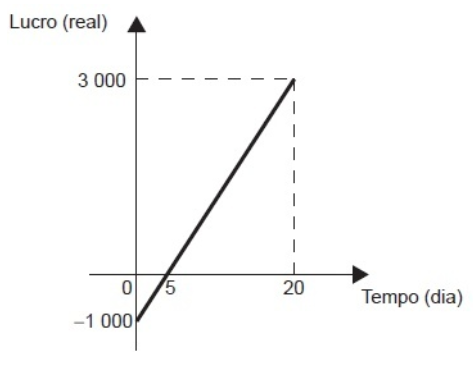
\includegraphics[scale=0.4]{imagens/q1.png}
        \end{column}
    \end{columns}

\end{frame}

\begin{frame}{UEA 2019}
    Ana e Beatriz caminham em uma pista retilínea, na mesma direção e sentido, e com as respectivas velocidades constantes. Sabe-se que a posição de Ana, $P_{A}$, é dada por $P_{A}(t) = 200 + 25t$, que a posição de Beatriz, $P_{B}$, é dada por $P_{B}(t) = 500 + 20t$ e que o tempo t é dado em minutos. Nessas condições, o tempo que Ana precisa para alcançar Beatriz é:

    \begin{enumerate}[a)]
        \item 60 minutos %
        \item 45 minutos
        \item 25 minutos
        \item 20 minutos 
        \item 40 minutos
    \end{enumerate}
\end{frame}

\begin{frame}{UEA 2019}
    No plano cartesiano, as representações das funções reais $f(x)=ax+2$ e $g(x)=-x+b$, com a e b números reais não nulos, passam pelo ponto $P(2,3)$. O valor de $f(-6)+g(2)$ é igual a:

    \begin{columns}
        \begin{column}{0.4\textwidth}
            \begin{enumerate}[a]
                \item 1
                \item 5
                \item 2 %
                \item 3
                \item 4
            \end{enumerate}
        \end{column}

        \begin{column}{0.6\textwidth}
            \centering
            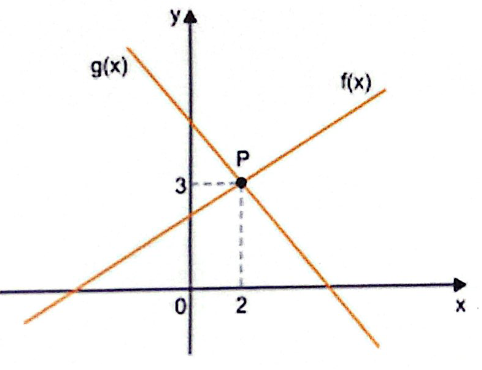
\includegraphics[scale=0.4]{imagens/q2.png}
        \end{column}
    \end{columns}

\end{frame}

\section{Função Quadrática}

\begin{frame}{ENEM 2013}
    
    A parte interior de uma taça foi gerada pela rotação de uma parábola em torno de um eixo z, conforme mostra a figura. A função real que expressa a parábola, no plano cartesiano da figura, é dada pela lei: $f(x)=\dfrac{3}{2}x^{2}-6x+c$ onde C é a medida da altura do líquido contido na taça, em centímetros. Sabe-se que o ponto V, na figura, representa o vértice da parábola, localizado sobre o eixo x. 

    \vfill
    \textbf{(continua no próximo slide)}
    
\end{frame}

\begin{frame}{ENEM 2013 (continuação)}
    Nessas condições, a altura do líquido contido na taça, em centímetros, é:
    \begin{columns}
        \begin{column}{0.4\textwidth}
            \begin{enumerate}[a)]
                \item $1$ 
                \item $2$  
                \item $4$
                \item $5$ 
                \item $6$ %
            \end{enumerate}
        \end{column}

        \begin{column}{0.6\textwidth}
            \centering
            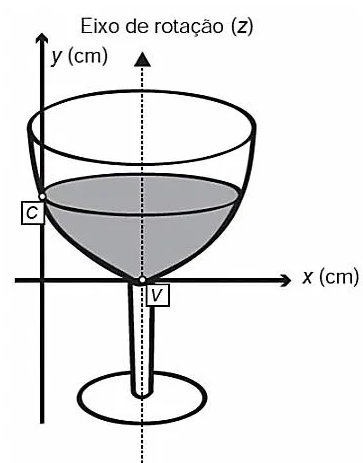
\includegraphics[width=0.7\linewidth]{imagens/enem 2013.png}
        \end{column}
    \end{columns}
    
\end{frame}

\begin{frame}{ENEM PPL 2019}
    No desenvolvimento de um novo remédio, pesquisadores monitoram a quantidade Q de uma substância circulando na corrente sanguínea de um paciente, ao longo do tempo t. Esses pesquisadores controlam o processo, observando que Q é uma função quadrática de t. Os dados coletados nas duas primeiras horas foram:

    \begin{center}
        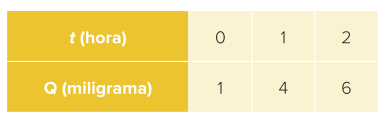
\includegraphics[scale=0.5]{imagens/enem-ppl-2019.png}
    \end{center} \textbf{(continua no próximo slide)}
\end{frame}

\begin{frame}{ENEM PPL 2019 (continuação)}
    Para decidir se devem interromper o processo, evitando riscos ao paciente, os pesquisadores querem saber, antecipadamente, a quantidade da substância que estará circulando na corrente sanguínea desse paciente após uma hora do último dado coletado. Nas condições expostas, essa quantidade (em miligrama) será igual a:

    \begin{enumerate}[a)]
        \item $4$
        \item $7$ %
        \item $8$ 
        \item $9$ 
        \item $10$ 
    \end{enumerate}
\end{frame}

\begin{frame}{UEA CG 2022}
    No plano cartesiano, o gráfico da função quadrática $f(x)=-6x^{2}+bx+c$, em que b e c são números reais, corta o eixo das abcissas nos pontos de coordenadas $(1,0)$ e $(3,0)$. O valor de $f(0)$ é:

    \begin{enumerate}[a]
        \item $-15$
        \item $-12$ 
        \item $-18$ %
        \item $-6$ 
        \item $-9$ 
    \end{enumerate}
\end{frame}

\begin{frame}{UEA - 2020}
    A figura mostra a representação gráfica, no plano cartesiano, da função $f(x) = x^{2}- bx+c$, com b e c números reais não nulos. Sabendo que os pontos P(2,0), Q(6,0) e (0, 12) pertencem à função f(x) e que a abcissa do ponto V é igual a ${b}/{2}$, as coordenadas do ponto V são:

    \begin{columns}
        \begin{column}{0.4\textwidth}
            \begin{enumerate}[a)]
                \item $(-2,4)$ 
                \item $(4,-2)$
                \item $(4,-4)$ %
                \item $(-4,4)$
                \item $(2,-4)$
            \end{enumerate}
        \end{column}

        \begin{column}{0.5\textwidth}
            \centering
            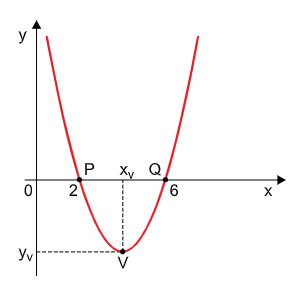
\includegraphics[width=0.8\linewidth]{imagens/uea-macro-2020.png}
        \end{column}
    \end{columns}
\end{frame}

\begin{frame}{UEA - 2017}
    O gráfico da função real $f(x)=ax^{2}+ bx + c$, com $a > 0$, é a parábola representada na figura. Sabendo-se que $x_{1}+x_{2}= -{b}/2$, onde $ x_{1}, x_ {2}$ são as raízes de $f(x) = 0$, é correto afirmar que a parábola intersecta o eixo das ordenadas no ponto:

    \begin{columns}
        \begin{column}{0.4\textwidth}
            \begin{enumerate}[a)]
                \item $(0,12)$ 
                \item $(12,0)$
                \item $(0,4)$ 
                \item $(0,16)$ %
                \item $(16,0)$
            \end{enumerate}
        \end{column}

        \begin{column}{0.5\textwidth}
            \centering
            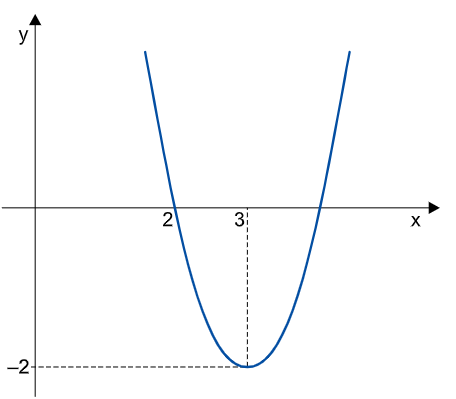
\includegraphics[width=0.8\linewidth]{imagens/uea-macro-2017(2).png}
        \end{column}
    \end{columns}
    
\end{frame}

\section{Função afim e função quadrática}
\begin{frame}{UEA - 2024}

    Considere as funções $f(x)={x}/{3}+b$ e $g(x)=x^{2}-bx+1$, em que b é um número real. Sabendo que $f(6)=4$, as coordenadas do vértice da parábola descrita pela função $g(x)$ são:

    \begin{enumerate}[a)]
        \item $(1,0)$ %
        \item $(-1,0)$
        \item $(-1,-1)$
        \item $(1,1)$ 
        \item $(0,-1)$
    \end{enumerate}

\end{frame}

\begin{frame}{2. UEA - 2019}
    Em um sistema de coordenadas cartesianas ortogonais estão representados os gráficos das funções f(x) e g(x), respectivamente, como uma reta e uma parábola de vértice V, que intercepta o eixo das abscissas no ponto M e na origem do sistema. Sabendo-se que $f(x) = 2x - 8$ e que os pontos M e V são comuns aos dois gráficos, as coordenadas do vértice V são:

    \begin{columns}
        \begin{column}{0.4\textwidth}
            \begin{enumerate}[a)]
                \item $(2,-4)$ %
                \item $(2,-8)$
                \item $(2,-6)$
                \item $(3,-8)$
                \item $(3,-6)$
            \end{enumerate}
        \end{column}

        \begin{column}{0.45\textwidth}
            \centering
            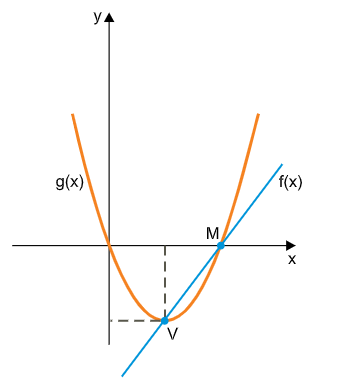
\includegraphics[width=0.8\linewidth]{imagens/uea-macro-2019.png}
        \end{column}
    \end{columns}
\end{frame}

\begin{frame}{5. UEA - 2018}
    Em um sistema de coordenadas cartesianas ortogonais estão representados os gráficos das funções $f(x) = x^{2}-4$ e $g(x) = –x^{2}+2x$, com os pontos comuns P e Q, conforme figura. As coordenadas dos pontos P e Q são, respectivamente,

    \begin{columns}
        \begin{column}{0.4\textwidth}
            \begin{enumerate}[a)]
                \item $(2,0)$ e $(-2,-3)$  
                \item $(2,0)$ e $(-0.5,-3)$
                \item $(1,0)$ e $(-1,-3)$ 
                \item $(2,0)$ e $(-1,-3)$ %
                \item $(1,0)$ e $(-0.5,-3)$
            \end{enumerate}
        \end{column}

        \begin{column}{0.5\textwidth}
            \centering
            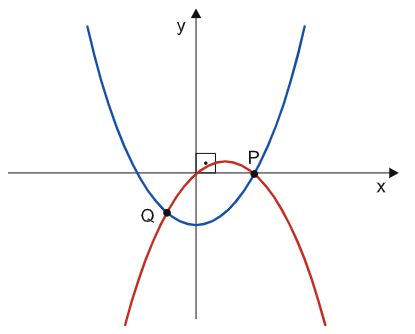
\includegraphics[width=0.8\linewidth]{imagens/uea-macro-2018.png}
        \end{column}
    \end{columns}
    
\end{frame}

\begin{frame}{12. UEA - 2024}
    Considere as funções $f(x)=({x}/{3})-b$ e $g(x)=x^{2}+bx+c$, em que b e c são números reais. Sabendo que $f(3)=-1$ e que $f(-3)=g(-2)$, o valor de $f(9)+g(2)$ é igual a:

    \begin{enumerate}[a)]
        \item 5
        \item 3
        \item 4
        \item 6 %
        \item 2
    \end{enumerate}
\end{frame}

\begin{frame}{6. ENEM 2022}

    Ao analisar os dados de uma epidemia em uma cidade, peritos obtiveram um modelo que avalia a quantidade de pessoas infectadas a cada mês, ao longo de um ano. O modelo é dado por $p(t)=-t^{2}+10t+24$, sendo t um número natural, variando de 1 a 12, que representa os meses do ano, e p(t) a quantidade de pessoas infectadas no mês t do ano. Para tentar diminuir o número de infectados no próximo ano, a Secretaria Municipal de Saúde decidiu intensificar a propaganda oficial sobre os cuidados com a epidemia. Foram apresentadas cinco propostas (I, II, III, IV e V), com diferentes períodos de intensificação das propagandas: $\textbf{(I)}\ 1 \leq t \leq 2, \textbf{(II)}\ 3 \leq t \leq 4, \textbf{(III)}\ 5 \leq t \leq 6, \textbf{(IV)}\ 7 \leq t \leq 9$ e $\textbf{(V)}\ 10 \leq t \leq 12$

    \vfill
    \textbf{(continua no próximo slide)}
\end{frame}
\begin{frame}{ENEM 2022 (continuação)}
    A sugestão dos peritos é que seja escolhida a proposta cujo período de intensificação da propaganda englobe o mês em que, segundo o modelo, há a maior quantidade de infectados. A sugestão foi aceita. A proposta escolhida foi a:

    \begin{enumerate}[a)]
            \item $I$
            \item $II$
            \item $III$ %
            \item $IV$ 
            \item $V$
        \end{enumerate}
\end{frame}

\begin{frame}{ENEM PPL 2018}
    A quantidade x de peças, em milhar, produzidas e o faturamento y, em milhar de real, de uma empresa estão representados nos gráficos, ambos em função do número t de horas trabalhadas por seus funcionários.

    \begin{center}
        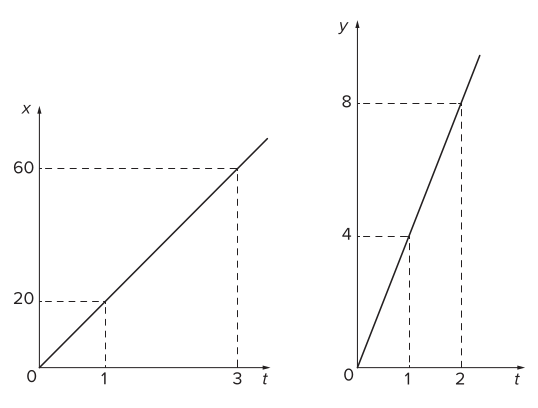
\includegraphics[scale=0.4]{imagens/enem-ppl-2018.png}
    \end{center}
    
\end{frame}

\begin{frame}{ENEM PPL 2018 (continuação)}
     O número de peças que devem ser produzidas para se obter um faturamento de R$\$\  10.000,00$ é:

    \begin{enumerate}[a)]
        \item 2000
        \item 2500
        \item 40000
        \item 50000 %
        \item 200000
    \end{enumerate}
\end{frame}


\section{Questões Extras}
\begin{frame}{9. Unifor-CE}
    Na figura abaixo têm-se os gráficos das funções quadráticas f e g. Se P é um dos pontos de interseção de f e g, então as suas coordenadas são:

    \begin{columns}
        \begin{column}{0.4\textwidth}
            \begin{enumerate}[a)]
                \item $(-{3}/{4},{57}/{16})$ 
                \item $(-{1}/{2},{9}/{4})$  %
                \item $(-{1}/{2},-{9}/{4})$
                \item $(-{1}/{4},{17}/{16})$ 
                \item $(-{1}/{4},-{17}/{16})$
            \end{enumerate}
        \end{column}

        \begin{column}{0.6\textwidth}
            \centering
            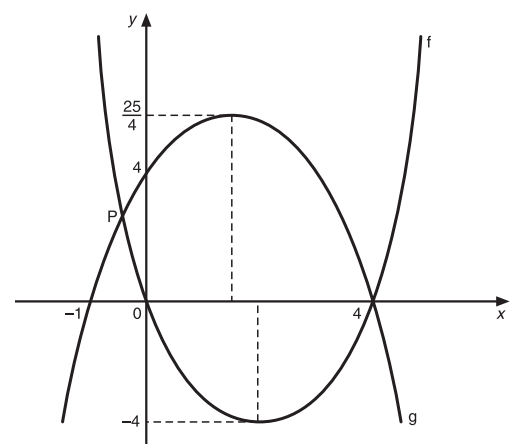
\includegraphics[width=0.9\linewidth]{imagens/Unifor-CE.png}
        \end{column}
    \end{columns}
    
\end{frame}

\begin{frame}{10. IFPE 2019}
    Um balão de ar quente sai do solo às 9h da manhã (origem do sistema cartesiano) e retorna ao solo 8 horas após sua saída, conforme demons- trado a seguir. A altura h, em metros, do balão, está em função do tempo t, em horas, através da fórmula $h(t)=(-{3}/{4})t^{2}+6t$ .

    \begin{center}
        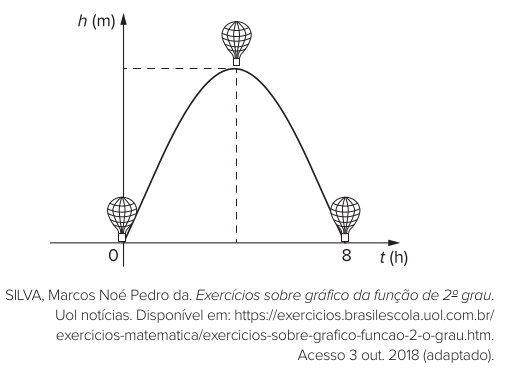
\includegraphics[scale=0.5]{imagens/IFPE 2019.png}
    \end{center}
\end{frame}

\begin{frame}{IFPE 2019 (continuação)}
    A altura máxima atingida pelo balão é de:

    \begin{enumerate}[a)]
        \item 21 m %
        \item 36 m
        \item 8 m 
        \item 4 m
        \item 12 m
    \end{enumerate}
\end{frame}

\begin{frame}{11. Fuvest 2022}
    Uma empresa construiu um poço para armazenar água de reúso. O custo para construir o primeiro metro foi de $R\$\ 1 000,00$, e cada novo metro custou $R\$\ 200,00$ a mais do que o imediatamente anterior. Se o custo total da construção foi de $R\$\ 48 600,00$, a profundidade do poço é:

    \begin{enumerate}[a)]
        \item 15 m
        \item 18 m %
        \item 21 m
        \item 24 m
        \item 17 m
    \end{enumerate}
\end{frame}

\begin{frame}{AFA}
    Para que o valor mínimo da função $y=x^{2}-4x+k$ seja igual a $-1$, o valor de k é:

    \begin{enumerate}[a)]
        \item 1
        \item 2
        \item 3 %
        \item 4
        \item 5
    \end{enumerate}
\end{frame}

\section{Gabarito}

\begin{frame}{Gabarito}
    \begin{columns}

    \column{0.48\textwidth}
    \begin{enumerate}
      \item A
      \item A
      \item C
      \item D
      \item D
      \item C
    \end{enumerate}

    \column{0.48\textwidth}
    \begin{enumerate}
      \setcounter{enumi}{6}
      \item B
      \item E
      \item B
      \item A
      \item B
      \item D
   
    \end{enumerate}

  \end{columns}
\end{frame}

\end{document}